\chapter{Reliability \& Operations for AI Systems}
\label{ch:reliability-ops}

\begin{quote}
\itshape
``An AI system that's 95\% accurate sounds great---until you realize that at 10,000 requests per hour, you're producing 500 wrong answers every hour, and you have no way to know which ones they are.''
\end{quote}

\vspace{0.5cm}

\noindent
Traditional SRE was built for deterministic systems. When a web server returns HTTP 500, something is clearly broken. When a database query times out, the dashboards light up. The entire discipline of Site Reliability Engineering---SLOs, error budgets, incident response, chaos engineering---assumes that systems either work correctly or fail visibly.

AI systems violate this assumption. An LLM can return a confident, well-formatted, completely wrong answer with an HTTP 200 and a latency of 150 milliseconds. Every monitoring dashboard shows green. The customer receives misinformation. And nobody knows until the support ticket arrives three days later.

This chapter covers the operational practices specific to AI systems: deployment strategies, monitoring for quality (not just uptime), incident response for probabilistic systems, and the cost management challenges that are unique to LLM-powered applications.


\section{Deployment Strategies for AI Systems}

AI systems have deployment characteristics that traditional CI/CD pipelines don't account for: non-deterministic outputs, model-version sensitivity, and the need for quality evaluation at deploy time. Figure~\ref{fig:ai-deployment} shows the three-stage deployment pipeline.

\begin{figure}[htbp]
\centering
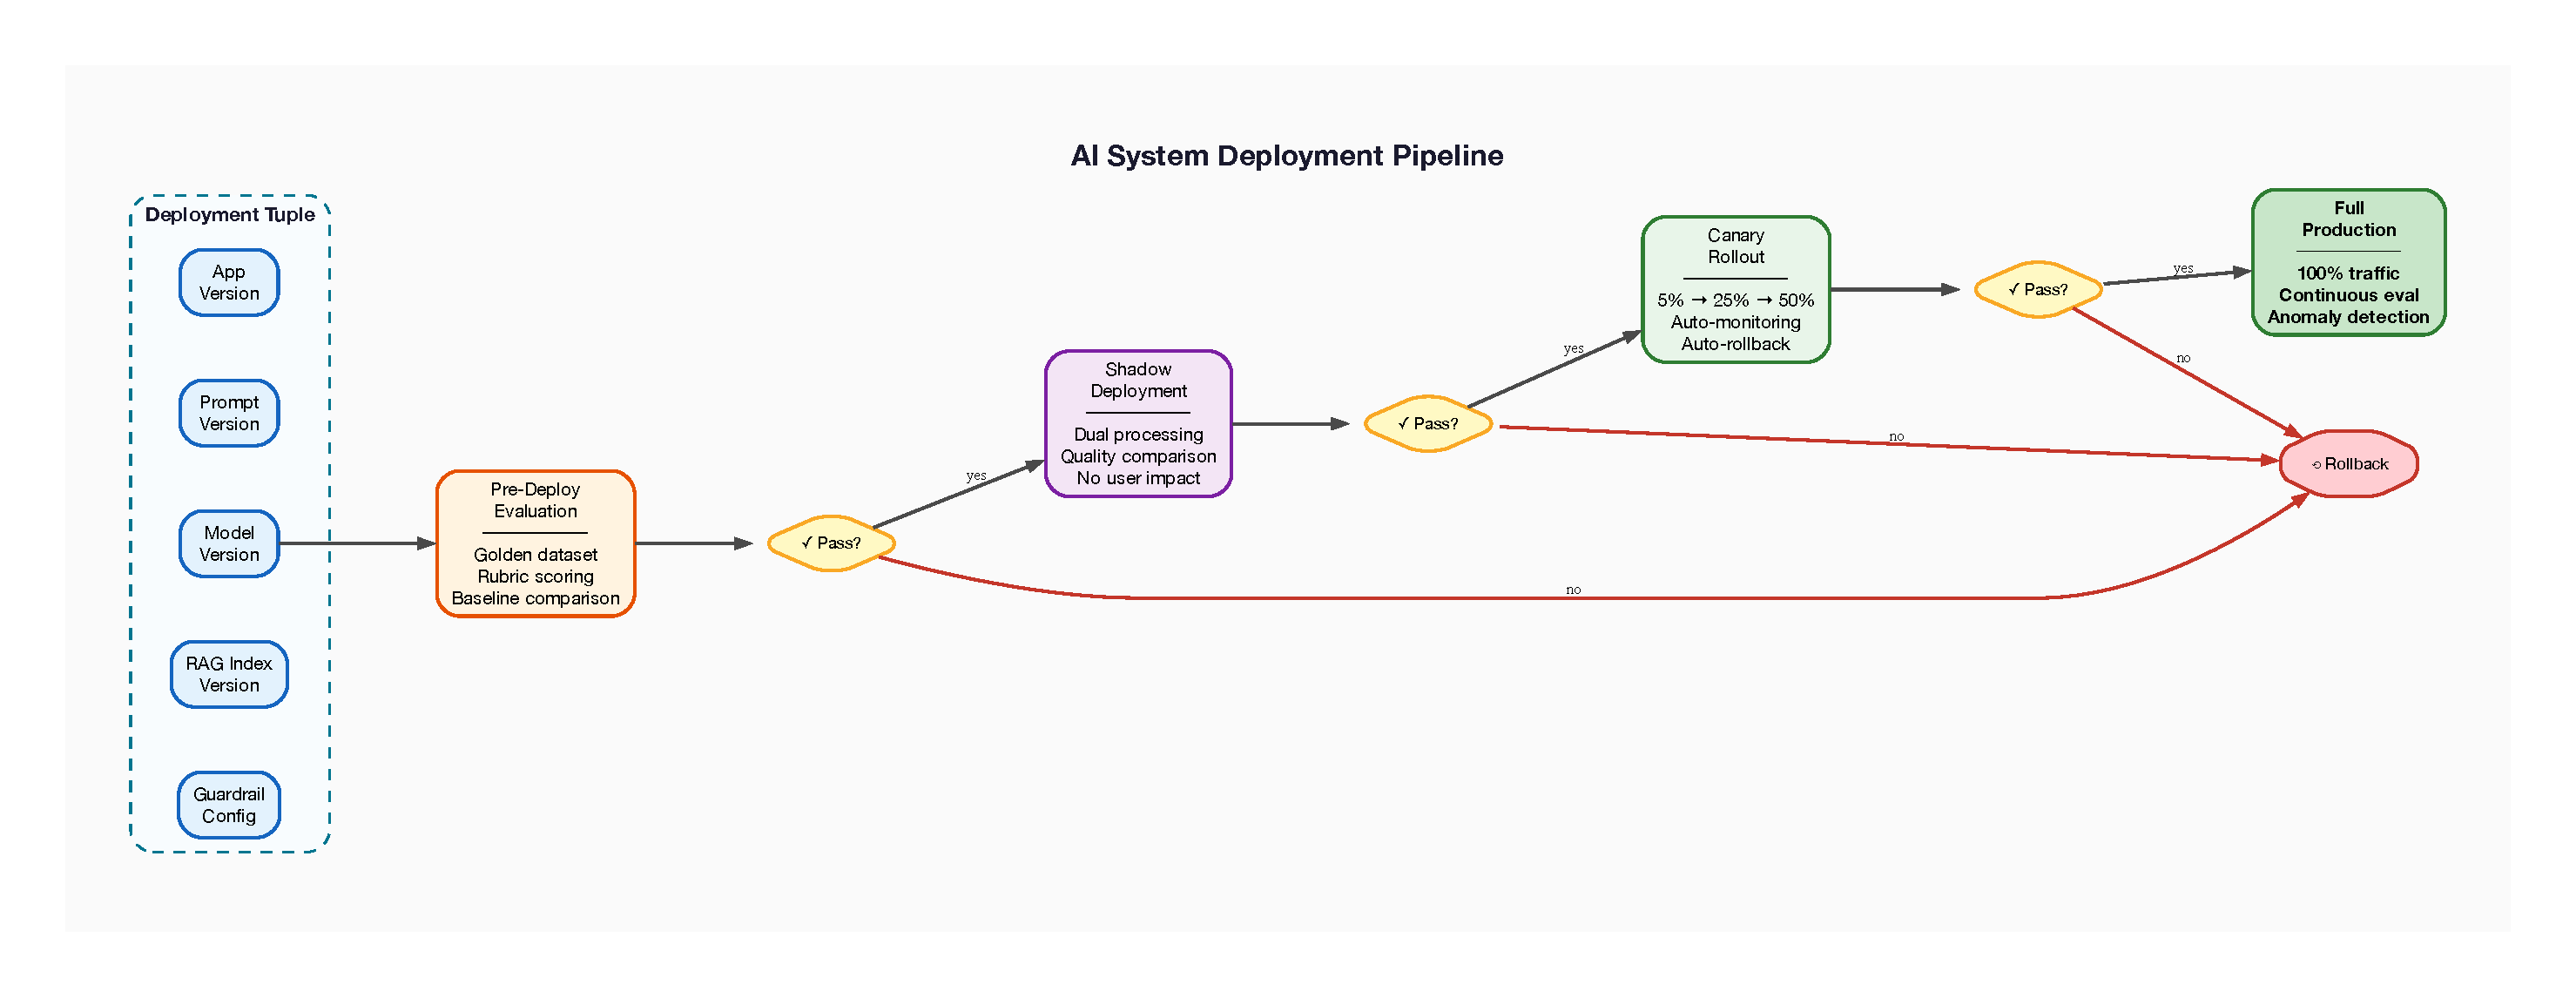
\includegraphics[width=\textwidth]{diagrams/compiled/ch11/ai-deployment-pipeline.pdf}
\caption{AI system deployment pipeline: evaluation gates, shadow deployment, and canary rollout with auto-rollback}
\label{fig:ai-deployment}
\end{figure}

\subsection{The AI Deployment Pipeline}

A production AI deployment pipeline has three stages beyond traditional software deployment:

\begin{enumerate}[leftmargin=*]
    \item \textbf{Pre-deployment evaluation}: Run the full golden dataset evaluation suite. Compare rubric scores against the locked baseline. Block deployment if any category regresses beyond the threshold (see Chapter~\ref{ch:evaluation-testing}).
    \item \textbf{Shadow deployment}: Deploy the new version alongside the current version. Both process real traffic; only the current version serves responses. Compare quality, latency, and cost.
    \item \textbf{Canary rollout}: Gradually shift traffic---5\% $\to$ 25\% $\to$ 50\% $\to$ 100\%---with automated quality monitoring at each step. Auto-rollback on quality regression.
\end{enumerate}

\subsection{What Gets Deployed}

An AI system deployment includes artifacts that traditional deployments don't:

\begin{itemize}[leftmargin=*]
    \item \textbf{Prompt versions}: System prompts, few-shot examples, output schemas. These are versioned independently of application code and deployed with the same rigor.
    \item \textbf{Model version pins}: The specific model version (e.g., \code{gpt-5.5-2026-04-15}), not the floating alias (\code{gpt-5.5}).
    \item \textbf{Evaluation baselines}: The expected rubric scores for the current configuration. These travel with the deployment so that production monitoring can compare against the correct baseline.
    \item \textbf{Guardrail configurations}: Safety filter thresholds, PII detection rules, content policy settings. These are configuration, not code, and require their own review process.
    \item \textbf{RAG index versions}: If the knowledge base has been updated, the new embedding index version must be deployed alongside the application changes.
\end{itemize}

\begin{tipbox}[The ``Deployment Tuple'']
Every AI system deployment should be described by a tuple: \code{(app\_version, prompt\_version, model\_version, index\_version, guardrail\_config)}. Any change to any element in this tuple is a deployment and must go through the evaluation pipeline. This is the single most important operational insight in this chapter: prompt changes are deployments.
\end{tipbox}


\section{Monitoring AI Systems in Production}

Traditional APM (Application Performance Monitoring) covers latency, throughput, and error rates. AI systems require an additional layer of monitoring for \emph{quality}---metrics that traditional tools do not capture. Figure~\ref{fig:monitoring-layers} illustrates the three-layer monitoring architecture.

\begin{figure}[htbp]
\centering
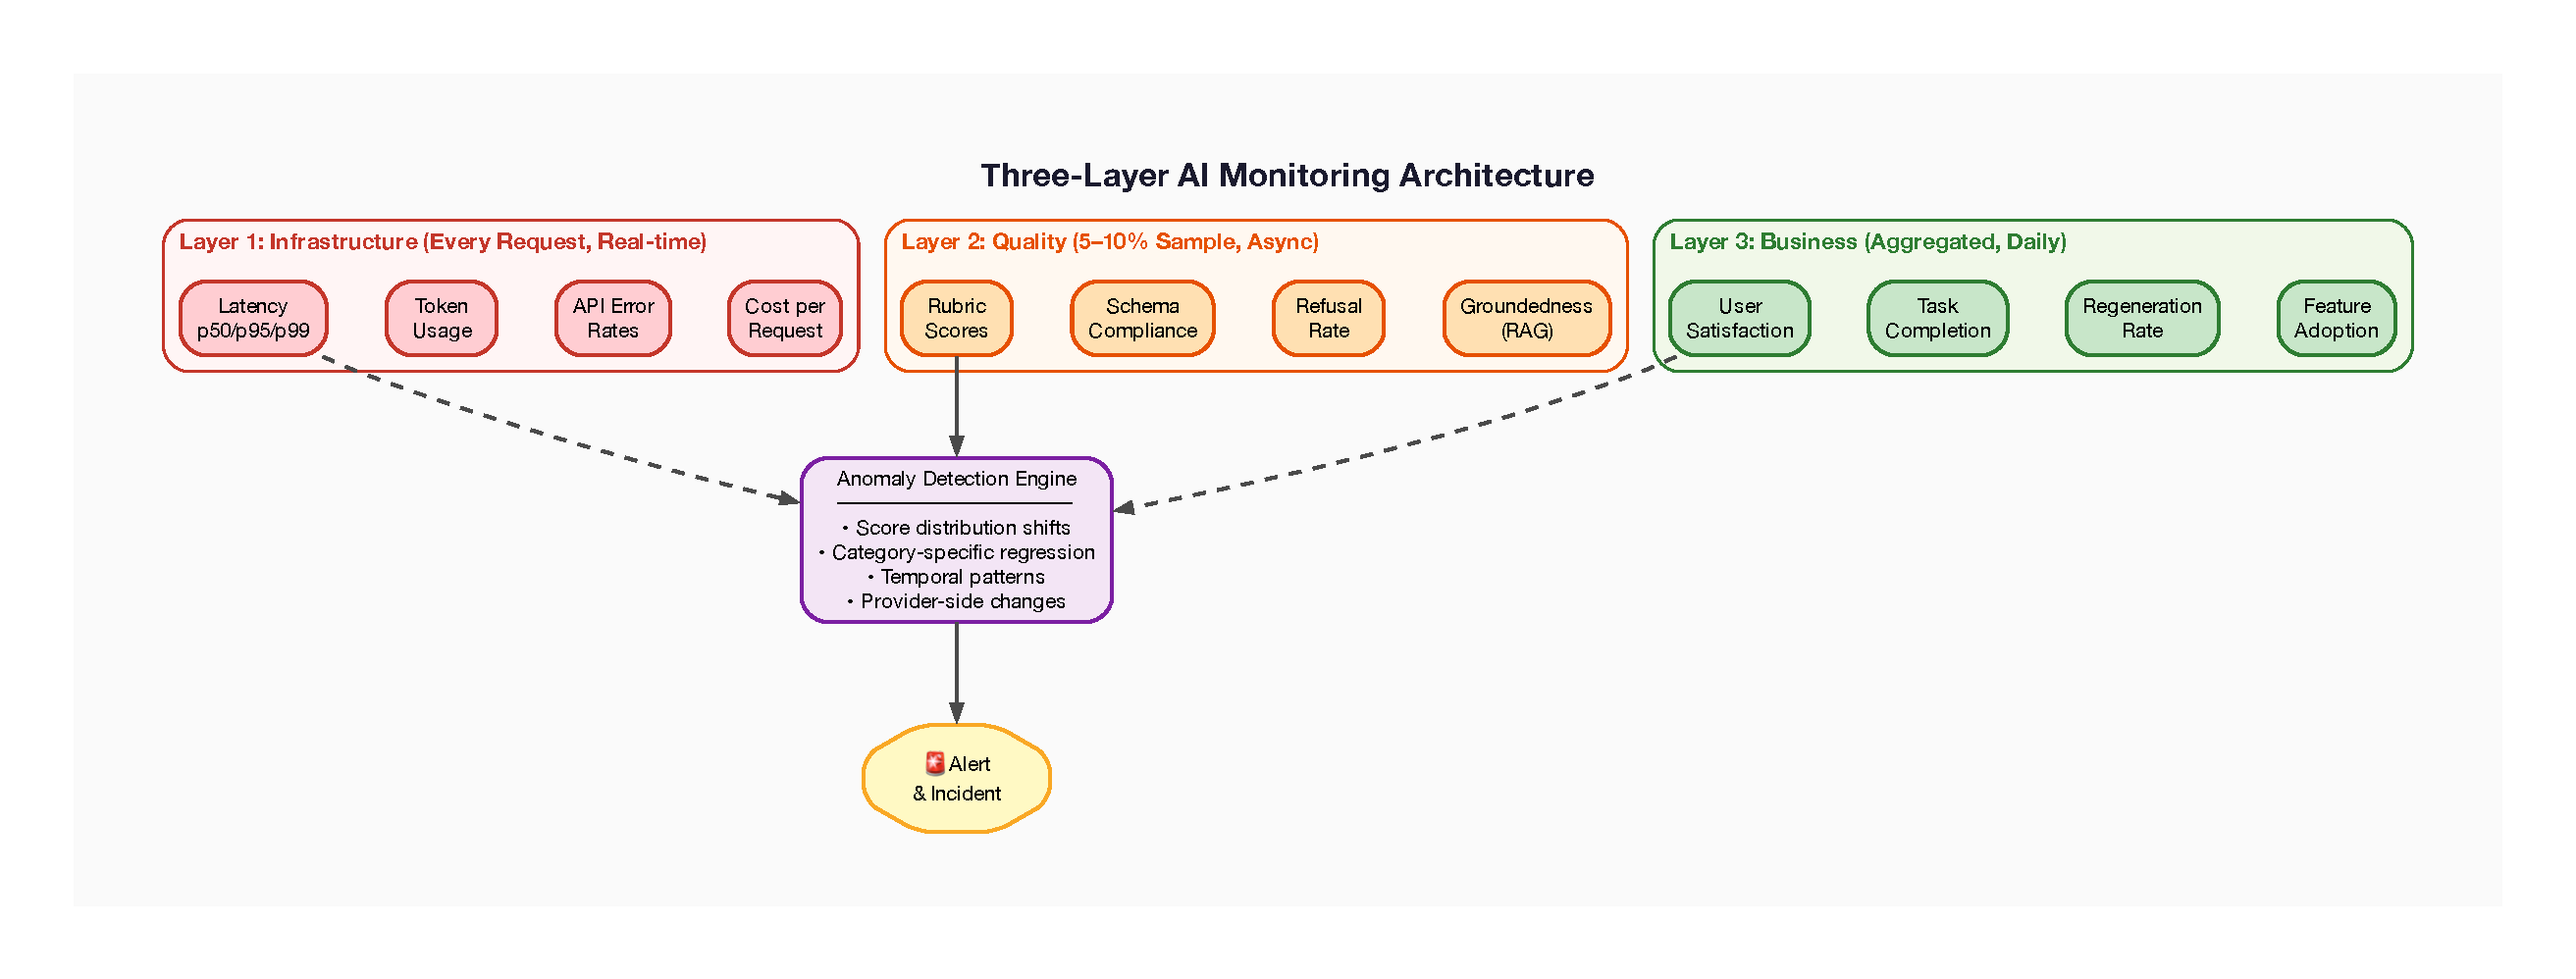
\includegraphics[width=\textwidth]{diagrams/compiled/ch11/monitoring-layers.pdf}
\caption{Three-layer AI monitoring: infrastructure (real-time), quality (sampled), and business (daily)}
\label{fig:monitoring-layers}
\end{figure}

\subsection{The Three Monitoring Layers}

\begin{enumerate}[leftmargin=*]
    \item \textbf{Infrastructure metrics} (every request, real-time):
    \begin{itemize}
        \item Latency: p50, p95, p99 by model and feature
        \item Token usage: Input and output tokens per request
        \item Error rates: API errors, timeouts, rate limits from model providers
        \item Cost: Dollars per request, aggregated by model and feature
    \end{itemize}
    
    \item \textbf{Quality metrics} (5--10\% sample, async):
    \begin{itemize}
        \item Rubric scores: Rolling averages per dimension (accuracy, completeness, relevance)
        \item Schema compliance: Percentage of outputs that parse and validate
        \item Refusal rate: How often the model declines to answer
        \item Groundedness: For RAG systems, percentage of claims grounded in source documents
    \end{itemize}
    
    \item \textbf{Business metrics} (aggregated, daily):
    \begin{itemize}
        \item User satisfaction: Thumbs up/down, NPS, support escalation rate
        \item Task completion: Percentage of user goals achieved (e.g., support tickets resolved)
        \item Regeneration rate: How often users ask for a new response (signal of dissatisfaction)
        \item Feature adoption: Usage trends by feature, user segment, time of day
    \end{itemize}
\end{enumerate}

\subsection{Anomaly Detection for AI Quality}

Traditional anomaly detection (z-scores, control charts) works for latency and throughput. AI quality metrics require domain-specific anomaly detection:

\begin{itemize}[leftmargin=*]
    \item \textbf{Score distribution shifts}: If the accuracy score distribution changes from unimodal (centered at 4.2) to bimodal (peaks at 2.0 and 4.5), a subset of inputs is being handled badly. This is invisible in aggregate averages.
    \item \textbf{Category-specific regression}: Overall quality may be stable while one category degrades. Monitor per-category scores with independent alert thresholds.
    \item \textbf{Temporal patterns}: Some quality issues appear only during peak hours (when batching is more aggressive), on weekends (when the input distribution shifts), or at month-end (when financial queries spike).
    \item \textbf{Provider-side changes}: Model providers update endpoints. Monitor for sudden changes in output characteristics (length, vocabulary, refusal rate) even when your code hasn't changed.
\end{itemize}


\section{Incident Response for AI Systems}

When an AI system fails, the incident response process is different from traditional software incidents.

\subsection{AI-Specific Incident Categories}

\begin{table}[htbp]
\centering
\caption{AI incident categories: detection, severity, and response patterns}
\label{tab:ai-incidents}
\begin{tabularx}{\textwidth}{p{2.8cm}p{2.8cm}X}
\toprule
\textbf{Category} & \textbf{Detection Signal} & \textbf{Response Pattern} \\
\midrule
Quality regression & Score drop $>$0.3 on rubric dimension & Compare against baseline; check for model/prompt changes; roll back if needed \\
\midrule
Hallucination spike & Groundedness ratio drops $>$5\% & Check RAG index freshness; verify retrieval quality; review source documents \\
\midrule
Prompt injection & Safety filter triggers or anomalous outputs & Activate adversarial monitoring; block affected input patterns; update guardrails \\
\midrule
Cost overrun & Token usage exceeds budget threshold & Check for prompt bloat; verify context assembly; enable circuit breaker \\
\midrule
Provider outage & API errors $>$5\% from model provider & Activate fallback model; route traffic to secondary provider; notify users of degraded quality \\
\midrule
RAG drift & Retrieval relevance scores decline & Rebuild embedding index; check for stale or corrupted documents; re-evaluate chunking \\
\bottomrule
\end{tabularx}
\end{table}

\subsection{The AI Incident Playbook}

\begin{enumerate}[leftmargin=*]
    \item \textbf{Identify}: Is this a quality issue or a systems issue? Systems issues (timeouts, errors) are handled traditionally. Quality issues (wrong answers, hallucinations) require the AI-specific playbook.
    \item \textbf{Scope}: How many users are affected? What categories of queries are impacted? Is this a regression across the board or specific to one input pattern?
    \item \textbf{Contain}: If the quality regression is severe, consider: switching to a fallback model, enabling stricter guardrails, or routing to human escalation for the affected category.
    \item \textbf{Diagnose}: Check the deployment tuple---did anything change? Model version, prompt version, RAG index, guardrail config? If nothing changed, the model provider may have updated their endpoint.
    \item \textbf{Remediate}: Fix the root cause. If it's a prompt issue, fix the prompt and run the evaluation suite before redeploying. If it's a model issue, switch to a pinned version or alternative provider.
    \item \textbf{Post-mortem}: Add the failure cases to your golden evaluation dataset. Update monitoring thresholds if the incident was detected late.
\end{enumerate}


\section{Cost Management}

LLM inference costs are a new category of operational expense that requires dedicated management.

\subsection{Cost Drivers}

\begin{itemize}[leftmargin=*]
    \item \textbf{Model selection}: Frontier models (GPT-5.5, Claude Opus 4.8) cost 10--50$\times$ more per token than fast models (Gemini 3.5 Flash, small open-source models). The Cognitive Router pattern (Chapter~\ref{ch:app-architecture}) is essential.
    \item \textbf{Context length}: Cost scales linearly with input tokens. Sloppy context assembly (including irrelevant documents in RAG) directly increases costs.
    \item \textbf{Retry loops}: The Validator-Corrector Proxy pattern increases reliability but multiplies costs during error states. Monitor retry rates closely.
    \item \textbf{Agent reasoning}: Autonomous agents can execute 10--50 LLM calls per task. Without budget limits (the Semantic Circuit Breaker), costs are unbounded.
    \item \textbf{Evaluation overhead}: LLM-as-Judge evaluation on production traffic costs 3--8\% of the production model's cost for 5\% sampling.
\end{itemize}

\subsection{Cost Optimization Strategies}

\begin{enumerate}[leftmargin=*]
    \item \textbf{Model routing}: Use the cheapest model that meets quality requirements. Route only complex queries to expensive models.
    \item \textbf{Prompt optimization}: Shorter prompts with higher information density reduce input token costs. Regularly audit prompt length.
    \item \textbf{Caching}: Semantic caching (Chapter~\ref{ch:app-architecture}) reduces API calls by 20--40\% for repetitive query patterns.
    \item \textbf{Batching}: Combine multiple requests into batch API calls during off-peak hours for non-real-time workloads (50--80\% cost reduction).
    \item \textbf{Self-hosting}: For high-volume, stable workloads, self-hosted open-source models (running on your own GPU infrastructure) can reduce per-token costs by 80--95\% after the initial hardware investment.
\end{enumerate}

\begin{cautionbox}[Denial of Wallet]
``Denial of Wallet'' is the AI equivalent of a DDoS attack: an adversary (or a buggy agent) generates a huge volume of expensive LLM calls, running up a massive bill. Defenses: per-user rate limits, per-session cost budgets, anomaly detection on spending patterns, and hard spending caps at the API gateway level.
\end{cautionbox}


\section{Graceful Degradation}

AI systems must degrade gracefully, not catastrophically. Design three tiers of service quality:

\begin{enumerate}[leftmargin=*]
    \item \textbf{Full service}: Primary model, full RAG context, complete evaluation pipeline. This is normal operation.
    \item \textbf{Degraded service}: Fallback model (cheaper, potentially lower quality), reduced RAG context (fewer documents retrieved), relaxed evaluation thresholds. Triggered by: primary model outage, cost budget exhaustion, or quality regression.
    \item \textbf{Static fallback}: Pre-computed responses for the most common queries, rule-based handling for simple requests, human escalation for everything else. Triggered by: complete model provider failure or severe budget constraints.
\end{enumerate}

\begin{keytakeaway}
Users tolerate a slightly worse AI response. They do not tolerate a blank screen, an error message, or a 30-second timeout. Design your fallback strategy so that the user always gets \emph{something} useful, even if it's not the best possible answer.
\end{keytakeaway}


\section{Operational Maturity Model}

\begin{table}[htbp]
\centering
\caption{AI operational maturity model: five levels from prototype to production excellence}
\label{tab:ai-maturity}
\begin{tabularx}{\textwidth}{lX}
\toprule
\textbf{Level} & \textbf{Characteristics} \\
\midrule
\textbf{L1: Prototype} & No evaluation suite. Manual testing. No cost tracking. Floating model versions. ``It works on my laptop.'' \\
\midrule
\textbf{L2: Deployed} & Basic golden dataset. CI/CD with evaluation gate. Cost alerts. Pinned model versions. Logs but no quality monitoring. \\
\midrule
\textbf{L3: Monitored} & Production quality monitoring (5\% sampling). Rubric-based evaluation. Anomaly detection. Defined incident playbook. Fallback model configured. \\
\midrule
\textbf{L4: Governed} & Model migration pipeline. Shadow deployment. Canary rollout. Per-feature cost tracking. Red-team testing cadence. Evaluation reviews. \\
\midrule
\textbf{L5: Excellent} & Automated regression detection. Multi-provider failover. Cost optimization pipeline. Continuous adversarial evaluation. Quality SLOs with error budgets. \\
\bottomrule
\end{tabularx}
\end{table}


\section{Chapter Summary}

\begin{enumerate}[leftmargin=*]
    \item \textbf{Prompt changes are deployments}: Every element of the deployment tuple (app, prompt, model, index, guardrails) must go through the evaluation pipeline
    \item \textbf{Monitor quality, not just uptime}: AI systems can fail silently. Three monitoring layers: infrastructure, quality (sampled), and business metrics
    \item \textbf{AI incidents are different}: Quality regressions, hallucination spikes, and prompt injection require specialized playbooks
    \item \textbf{Cost is a first-class operational concern}: Model routing, caching, batching, and self-hosting are essential cost levers
    \item \textbf{Design for graceful degradation}: Three tiers of service quality, from full service to static fallback
    \item \textbf{Aim for operational maturity L3+}: Production quality monitoring, rubric evaluation, anomaly detection, and defined incident playbooks
\end{enumerate}
